\section{Evaluation}
We collected data from $10$ subjects, each using our instrumented visualization for approximately $50$ minutes on a series of structured and unstructured tasks. We used the collected data to test the validity and effectiveness of collecting eye-tracking data in visualization space in two ways. First, we used the system described in Section~\ref{sec:Methods} to investigate whether viewed objects detected by our instrumentation align with the tasks we asked people to do. We found that it does, and believe this provides strong evidence, albeit not definite, that our method works. Second, we quantitatively compared the results produced by our automatic instrumentation, to annotations produced by human coders. Specifically, we compared the similarity of our results to human annotations, with the similarity between human annotations. We found that our results are on average as similar to human annotation as are human annotations are similar to each other. Finally, we repeated this quantitative analysis for viewing scores computed without the prediction component, and found that detection accuracy dropped on average by $5\%$. 

\subsection{Study Design }

\textbf{Setup: } We used a lightweight $60$Hz EyeX eye-tracker from Tobii. Subjects used a 17'' monitor and were seated approximately $30''$ away from it.

\textbf{Subjects:} We collected data from $10$ graduate and undergraduate students with ages ranging between $20$ years and $30$ years. Seven of them were male and three were female. Subjects were paid $10$ for their time.

\textbf{Protocol:} Subjects were first given a description of the study's purpose and protocol. They were then introduced to our IMDB PivotPaths visualization and asked to perform a few training tasks to help them get accustomed with the visualization. This introductory part lasted approximately $10$ minutes on average. The main section of the study followed, involved multiple instances of five types of tasks, and lasted approximately $50$ minutes. 


\textbf{Tasks:} We asked subjects to complete six types of tasks, the first of which was used during the training session. We aimed to balance structured tasks and unstructured tasks. To solve the structured tasks, subjects had to consider a set of objects that was better defined and less variable than in unstructured tasks. This made it easier for us to test the degree to which our detection of viewed objects is aligned with the data required to complete the tasks. On the other hand, data collected for unstructured tasks may be better at informing designs of future analysis systems of such data. We limited the time we allowed subjects to spend on each task for two reasons: to limit the total duration of the study, and to make results comparable across time and users.

\begin{itemize}
	\item \textbf{Task1 (Training):} Providing information about an actor (e.g.: top ranked movie, most worked with director).
	\item \textbf{Task2:} Finding four commonalities between pairs of movies (e.g., Raiders of the Lost Ark and Indiana Jones and the Last Crusade). Subjects solved four instances of this task, limited at three minutes each.  We considered this to be a structured task.
	\item \textbf{Task3:} Ranking collaborations between a director and three actors (e.g., Judd Apatow with Seth Rogen, Paul Rudd, Jonah Hill). Subjects solved four instance of this task, at two minutes each. We considered this to be a structured task.
	\item \textbf{Task4:} Given three movies, subjects were asked to recommend a fourth (e.g., Avatar, Titanic, Looper). Subjects solved three such tasks, each in $5$ minutes. We considered this to be a semi-structured task.
	\item \textbf{Task5:} Exploratory task: given a brief and incomplete description of the ``Brat Pack'', a group of young actors popular in the 80's, subjects were asked to find additional members and movies they acted in. Subjects solved one such task, in approximately $5$ minutes. We considered this an unstructured task.
\end{itemize}


\subsection{Results}
\label{sec:EvalResults}
\textbf{Qualitative analysis: } First, we analyzed results using the system described in Section~\ref{sec:Methods}. The top of Figure~\ref{fig:heatmap} shows data for the first four tasks aggregated over all ten users. The four clusters noticeable in the heatmap provide a first indication that elements viewed by users are in tight correlation with the four tasks they had to do, which is in accordance with our hypothesis and expectation. However, the four different clusters appearing in the heatmap are not sufficiently telling, since the views involved in each task were distinct and showed different data. As such, even a random sampling of objects from these views could produce a similar high level clustering in the heatmap. 

\begin{figure*}[htb]
  \centering
  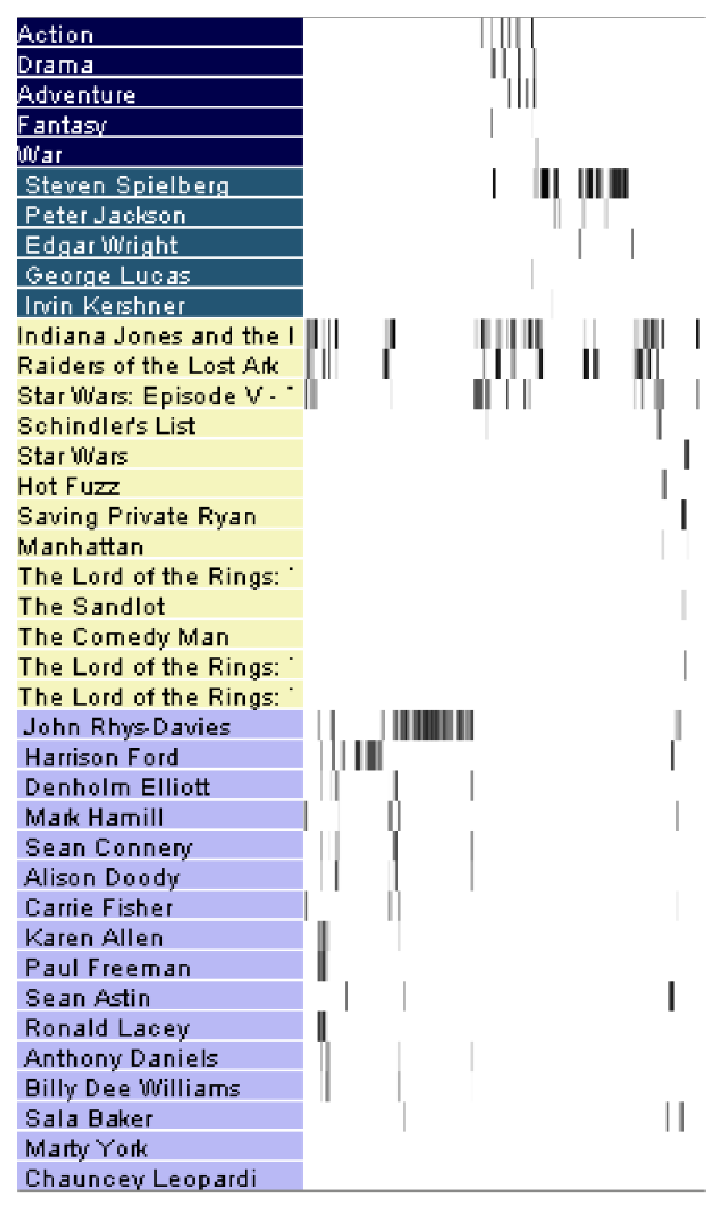
\includegraphics[width=\linewidth]{images/heatmap.eps}
  \caption{(Top) Aggregated data for all ten users reveals three clusters of viewed objects corresponding to the first three tasks that subjects were asked to do. (Middle) Sorting the heatmap by how much each object was viewed shows, as hypothesized, that objects most relevant to the task, finding commonalities between Raiders of the Lost Ark and Indiana Jones and the Last Crusade, were viewed most often. (Bottom) Sorting the heatmap by which objects were viewed first, reveals interesting temporal patterns for a particular user. }
	\label{fig:heatmap}
\end{figure*}

A closer look at the specific data objects listed in the heatmap, as well as their associated viewing activity, removes this concern. In Figure~\ref{fig:heatmap} middle, we restricted the heatmap to showing only data corresponding to the second task subjects completed, which was finding the similarities between the movies ``Raiders of the Lost Ark'' and ``Indiana Jones and the Last Crusade''. The view involved in solving this task contained about $70$ actors, $16$ movies, $11$ directors, and $15$ genres, yet the heatmap reveals that only a small subset of these elements were viewed regularly, and that the more connected the data element was to the task, the more often and intently it was viewed.

Moreover, looking at the data for a single user, sorted by first view, (Figure~\ref{fig:heatmap}) bottom, reveals temporal patterns in how the subject solved the task: they looked at movie titles throughout the task, though predominantly in the beginning, actors in the first half, in a fairly consistent sweep, and directors and genres in the second half. 

\textbf{Quantitative analysis:} Second, we compared lists of viewed objects produced by our instrumentation to similar lists created manually by human coders who visually inspected screen shots tougher with gaze positions. To this end, we enlisted the help of four coders and asked them to code data corresponding to one task of approximately two minutes, for two subjects. The two subjects were selected randomly and were the same for all four coders. 

Coders were asked to indicate what they thought the subjects looked at, and note the start and end time of each object's viewing, at a resolution of $100$ms. They were allowed to indicate multiple objects if they were unsure which of those objects was viewed. Coders used the screen shot part of the application described in Section~\ref{sec:Methods}, advanced through the data in $100$ms increments, and annotated it as requested. Each coder spent approximately one hour on each of the two subjects.

We transformed the data provided by each coder for each user into a long vector with a position for each $100$ms that was analyzed, and their coding result for that particular $100$ms interval. We then created a heatmap at a resolution of $100$ms, and for each column recorded the visual object with the highest score at that particular time. This yielded a vector of the same form to that obtained from our coders' data.  

We defined a similarity measure between two such vectors as the percentage of temporally aligned cells from the two vectors that are equal. Equality between cells was defined as a non-empty intersection between their contents. Finally, we computed such similarities between each coder and the automatically generated annotation for each of the two users ($4$ coders $\times$ $2$ subjects $\times$ $1$ automated annotation $=$ $8$ similarities), and similarities between all pairs of coders for each subject ($6$ coder pairs $\times$ $2$ subjects $=$ $12$ similarities). These similarities are shown in Figure~\ref{fig:quantitative}. As can be seen, the similarities between the results of human coders and our instrumentation are very close to the similarities between coders. 

\begin{figure}[htb]
  \centering
  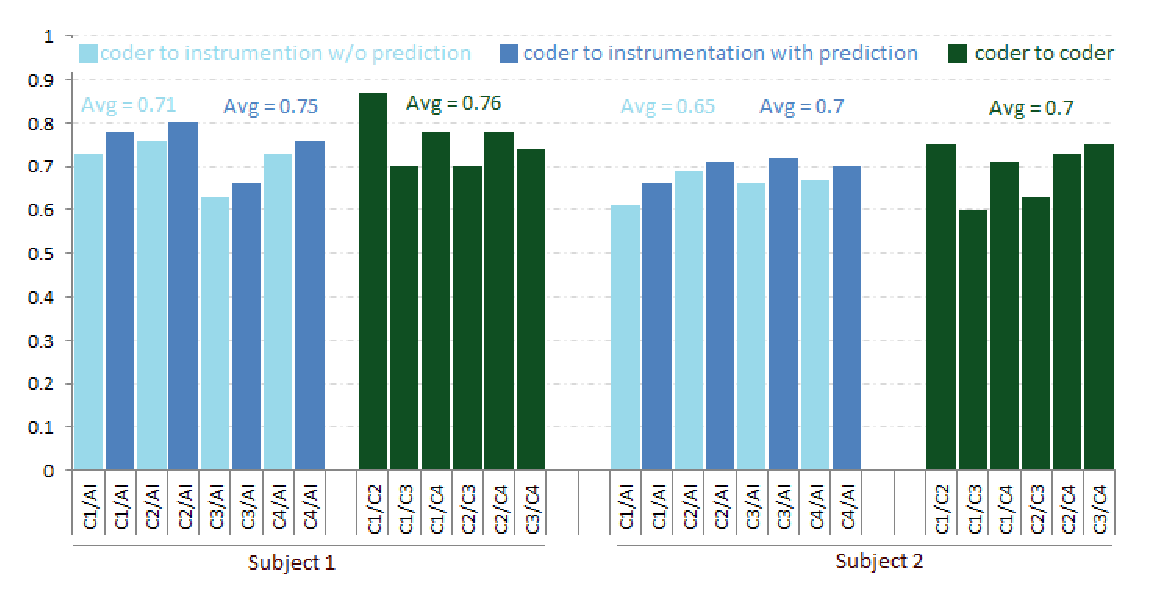
\includegraphics[width=\linewidth]{images/quantitative.eps}
  \caption{Similarities of viewing scores computed with viewed object prediction (dark blue), and without prediction (light blue) to annotations by four human coders (C1-4), are compared to similarities between the human coders own results (green), for two subjects. }
	\label{fig:quantitative}
\end{figure}

Finally, since we captured viewing scores ($vs$), gaze scores ($gs$), and prediction scores ($ps$) separately, we were able to assess the effectiveness of our ``intelligent gaze interpretation'' algorithm by re-running the quantitative analysis using viewing scores that were computed without the prediction component. As shown in Figure~\ref{fig:quantitative}, we found that the prediction component improves accuracy by approximately $5\%$. 